\documentclass[11pt]{article}
\usepackage{amsmath,amsthm,amssymb,amsfonts}
\usepackage{enumerate}
\usepackage{color}
\usepackage[margin=1in, top=.5in]{geometry}
\usepackage{float}
\usepackage[parfill]{parskip}

\usepackage{tikz}
\usetikzlibrary{graphs, graphs.standard,arrows}

\DeclareMathOperator*{\argmin}{arg\,min}
\DeclareMathOperator*{\argmax}{arg\,max}
\DeclareMathOperator*{\adjoint}{ad}

 
\newcommand{\N}{\mathbb{N}}
\newcommand{\Z}{\mathbb{Z}}
\newcommand{\C}{\mathbb{C}}
\newcommand{\Q}{\mathbb{Q}}
\newcommand{\R}{\mathbb{R}}
\newcommand{\norm}[1]{\left\lVert#1\right\rVert}

\newcommand{\pose}[2]{{}^{#1}T_{#2}}

\newenvironment{problem}[2][Problem]{\begin{trivlist}
\item[\hskip \labelsep {\bfseries #1}\hskip \labelsep {\bfseries #2.}]}{\end{trivlist}}
%If you want to title your bold things something different just make another thing exactly like this but replace "problem" with the name of the thing you want, like theorem or lemma or whatever

%%This optional package allows you to use TikZ to typeset automata
%\usepackage{tikz}
%\usetikzlibrary{automata}
%
%%This optional package allows you to use xypic to typeset automata
%\usepackage[all]{xy}
%
%%This optional package allows you to include external graphics
\usepackage{graphicx}

%%%%%%%%%%%%%%%%%%%%%%%%%%%%%%%%%%%%%%%%%%%%%%%%%%%%%%%%%%%%%%%%%%%%%%%%%%%%%
%%%%    FILL THESE FIELDS IN
%%%%%%%%%%%%%%%%%%%%%%%%%%%%%%%%%%%%%%%%%%%%%%%%%%%%%%%%%%%%%%%%%%%%%%%%%%%%%

\title{Visual Inertial Odometry}
\author{Martin Deegan}
 
\begin{document}
 
\maketitle
\tableofcontents

\section{Vertices}
\subsection{State Vertex}
At each timestamp, $t$, we track the state of the vehicle. This includes any pose information as well as varying parameters in sensors or the world which we need to keep track of.




\subsubsection{Pose}
We track the pose in the lie group as well as its first and second derivatives in the lie algebra.

\begin{align}
	X_t &\in SE(3)\\
	\dot X_t &\in \mathfrak{se}(3)\\
	\ddot X_t &\in \mathfrak{se}(3)
\end{align}

Since $\mathfrak{se}(3)$ is isomorphic to $\R^6$, we will use the $\R^6$ notion from now on.

\subsubsection{IMU biases}
We track the varying biases of the IMU. These are tracked within the IMU's frame.

\begin{align}
	b_g &\in \R^3\\
	b_a &\in \R^3
\end{align}

~\\\\\\

The state at time $t$ will be represented simply by $x_t$.
\begin{figure}[H]
	\centering
	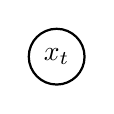
\begin{tikzpicture}
	\begin{scope}[every node/.style={circle,thick,draw}]
	\node (A) at (0, 0) {$x_t$};
	\end{scope}
	\end{tikzpicture}
	\caption{When displayed as a graph, a state vertex will have this form.}
\end{figure}

\subsection{World Parameters}
Gravity

\begin{align}
	g \in \R^3
\end{align}

\subsection{Camera Intrinsic Parameters}

\begin{align}
	K &= \begin{bmatrix}
	\frac{1}{p_x} & 0 & c_x\\
	0 & \frac{1}{p_y} & c_y\\
	0 & 0 & 1
	\end{bmatrix}\begin{bmatrix}
	f & 0 & 0 & 0\\
	0 & f & 0 & 0\\
	0 & 0 & 1 & 0
	\end{bmatrix}
\end{align}
\subsection{IMU Intrinsic Parameters}
Due to small mechanical errors in the manufacturing process, the axes of gyroscopes and accelerometers may not be perfectly orthogonal. These errors are proportional to the magnitude of the signal. An acrobatic drone will undergo large accelerations and angular rates and therefore, it is important to estimate these misalignments and correct for them.

The intrinsics we store are 3 by 3 mixing matrices. Ideally, these should be close to zero.
\begin{align}
	L_g \in \R^{3\times 3}\\
	L_a \in \R^{3\times 3}
\end{align}

\subsection{Extrinsic Parameters}
The main goal of our visual odometry is to estimate the pose of the center of mass of our robot for feedback control. We want the center of mass because rotations performed by the vehicle will be about that point.




In order to do that, we need to know the relative poses of our IMU and camera. We have 3 reference frames on the vehicle: center of mass ($\mathcal F_o$), camera ($\mathcal F_c$) , and IMU ($\mathcal F_i$). We need to keep track of the rigid transformations between them, $\pose{i}{o}$ and $\pose{c}{o}$. The adjoint will especially helpful in converting the first and second derivatives into different reference frames.

\begin{figure}[H]
	\centering
	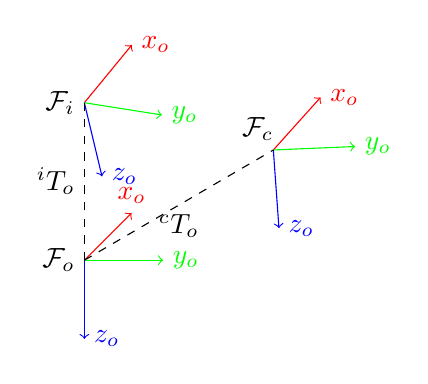
\begin{tikzpicture}[x=1cm, y=1cm, z=-0.6cm]
	% Center of mass frame
	\draw [red, ->] (0, 0, 0) -- (0, 0, -1) node [above] {$x_o$};
	\draw [green, ->] (0, 0, 0) -- (1, 0, 0) node [right] {$y_o$};
	\draw [blue, ->] (0, 0, 0) -- (0, -1, 0) node [right] {$z_o$};
	\draw [dashed] (0, 0, 0) -- (0, 0, 0) node [left] {$\mathcal{F}_o$};
	
	% Camera frame
	\draw [red, ->] (0, -1, -4) -- (0.002, -0.93, -4.997) node [right] {$x_o$};
	\draw [green, ->] (0, -1, -4) -- (0.997, -0.998, -4.07) node [right] {$y_o$};
	\draw [blue, ->] (0, -1, -4) -- (0.07, -1.995, -4.002) node [right] {$z_o$};
	\draw [dashed] (-0.2, -1, -4) -- (-0.2, -1, -4) node [above] {$\mathcal{F}_c$};
	% IMU frame
	\draw [red, ->] (0, 2, 0) -- (0.009, 2.14, -0.99) node [right] {$x_o$};
	\draw [green, ->] (0, 2, 0) -- (0.99, 1.85, 0.009) node [right] {$y_o$};
	\draw [blue, ->] (0, 2, 0) -- (0.14, 0.98, -0.14) node [right] {$z_o$};
	\draw [dashed] (0, 2, 0) -- (0, 2, 0) node [left] {$\mathcal{F}_i$};
	
	\draw [black, dashed] (0, 0, 0) -- (0, -1, -4) node [midway, below] {$\pose{c}{o}$};
	\draw [black, dashed] (0, 0, 0) -- (0, 2, 0) node [midway, left] {$\pose{i}{o}$};
	\end{tikzpicture}
	\caption{The 3 reference frames on the vehicle. Note: we use the North, East, Down (NED) convention.}
\end{figure}

\begin{align}
	\pose{i}{o} &\in SE(3)\\
	\pose{c}{o} &\in SE(3)\\
	\text{Ad}_{\pose{i}{o}} &\in \R^{6 \times 6}\\
	\text{Ad}_{\pose{c}{o}} &\in \R^{6 \times 6}
\end{align}

\section{Factors}
\subsection{State Prior Factors}
State prior factors are mono factors which act on the oldest state vertex in the sliding window. We can marginalize state vertices which leave the sliding window and we can marginalize feature points out as they leave our working area. These can be marginalized into a single prior for the system.

\subsection{IMU}
The IMU is running at a much higher frequency than the camera. We can pre-integrate the IMU measurements into a single transformation between state vertices.

\subsection{Vision Factors}
Using projective geometry to track feature in the world. Possibly ORB features.

\subsection{Zero Velocity Factors} 
When we know the vehicle is on the ground (such as on start), we can add zero velocity factors which constrain angular and linear velocities. This will allow us to quickly observe gyroscope bias.
\subsection{Tracking Camera Factors}

\subsection{GPS Factors}

\section{Calibration}
We have many parameters to calibrate on our system. Namely, our sensor intrinsics and extrinsics. We can break down our calibration into stages to restrict our nonlinear least squares optimization problem to fewer variable. This will speed up calibration speeds as well as improving the solution (assuming previous steps have good solutions).

\subsection{Setup}
Calibration should take place in a motion tracking environment such as a Qualisys, Optitrack, or Vicon camera system.

There should be a checkerboard for camera intrinsics calibration.
\begin{figure}[H]
\centering

\includegraphics[width=0.5\textwidth]{checkerboard}
\end{figure}

\subsection{Camera Intrinsics Calibration}

\subsection{Gyro Bias Calibration}
\subsection{Final Calibration}
\end{document}